This section covers basic performance tests, i.e. how specific algorithms scale in parallel with increasing \emph{number of processors}. So far, all calculations for this research were conducted on the Lichtenberg high performance computer of the TU Darmstadt.

\section{Weak scaling - XdgPoisson}
Weak scaling is investigated of the test problem introduced in \ref{sec:XdgPoisson}. This means the problem size per processor is constant during the study (in this case approximately 10.000 DOF / core). So the total problem size grows with increasing number of cores. The expectation is that wall clock time remains constant trough the study. This means in the same time frame with $N$ cores we are able to solve a system, which is $N$ times the size of a single core run.

In \ref{weakXdgPoissonScaling} the scaling of V-krylov-cycle is shown:

\subsection{solver scaling}

\graphicspath{{./apdx-MPISolverPerformance/weakScaling/XdgPoisson/plots/}} 
\begin{figure}[h!]
	\begin{center}
		% GNUPLOT: LaTeX picture with Postscript
\begingroup
  \makeatletter
  \providecommand\color[2][]{%
    \GenericError{(gnuplot) \space\space\space\@spaces}{%
      Package color not loaded in conjunction with
      terminal option `colourtext'%
    }{See the gnuplot documentation for explanation.%
    }{Either use 'blacktext' in gnuplot or load the package
      color.sty in LaTeX.}%
    \renewcommand\color[2][]{}%
  }%
  \providecommand\includegraphics[2][]{%
    \GenericError{(gnuplot) \space\space\space\@spaces}{%
      Package graphicx or graphics not loaded%
    }{See the gnuplot documentation for explanation.%
    }{The gnuplot epslatex terminal needs graphicx.sty or graphics.sty.}%
    \renewcommand\includegraphics[2][]{}%
  }%
  \providecommand\rotatebox[2]{#2}%
  \@ifundefined{ifGPcolor}{%
    \newif\ifGPcolor
    \GPcolortrue
  }{}%
  \@ifundefined{ifGPblacktext}{%
    \newif\ifGPblacktext
    \GPblacktexttrue
  }{}%
  % define a \g@addto@macro without @ in the name:
  \let\gplgaddtomacro\g@addto@macro
  % define empty templates for all commands taking text:
  \gdef\gplbacktext{}%
  \gdef\gplfronttext{}%
  \makeatother
  \ifGPblacktext
    % no textcolor at all
    \def\colorrgb#1{}%
    \def\colorgray#1{}%
  \else
    % gray or color?
    \ifGPcolor
      \def\colorrgb#1{\color[rgb]{#1}}%
      \def\colorgray#1{\color[gray]{#1}}%
      \expandafter\def\csname LTw\endcsname{\color{white}}%
      \expandafter\def\csname LTb\endcsname{\color{black}}%
      \expandafter\def\csname LTa\endcsname{\color{black}}%
      \expandafter\def\csname LT0\endcsname{\color[rgb]{1,0,0}}%
      \expandafter\def\csname LT1\endcsname{\color[rgb]{0,1,0}}%
      \expandafter\def\csname LT2\endcsname{\color[rgb]{0,0,1}}%
      \expandafter\def\csname LT3\endcsname{\color[rgb]{1,0,1}}%
      \expandafter\def\csname LT4\endcsname{\color[rgb]{0,1,1}}%
      \expandafter\def\csname LT5\endcsname{\color[rgb]{1,1,0}}%
      \expandafter\def\csname LT6\endcsname{\color[rgb]{0,0,0}}%
      \expandafter\def\csname LT7\endcsname{\color[rgb]{1,0.3,0}}%
      \expandafter\def\csname LT8\endcsname{\color[rgb]{0.5,0.5,0.5}}%
    \else
      % gray
      \def\colorrgb#1{\color{black}}%
      \def\colorgray#1{\color[gray]{#1}}%
      \expandafter\def\csname LTw\endcsname{\color{white}}%
      \expandafter\def\csname LTb\endcsname{\color{black}}%
      \expandafter\def\csname LTa\endcsname{\color{black}}%
      \expandafter\def\csname LT0\endcsname{\color{black}}%
      \expandafter\def\csname LT1\endcsname{\color{black}}%
      \expandafter\def\csname LT2\endcsname{\color{black}}%
      \expandafter\def\csname LT3\endcsname{\color{black}}%
      \expandafter\def\csname LT4\endcsname{\color{black}}%
      \expandafter\def\csname LT5\endcsname{\color{black}}%
      \expandafter\def\csname LT6\endcsname{\color{black}}%
      \expandafter\def\csname LT7\endcsname{\color{black}}%
      \expandafter\def\csname LT8\endcsname{\color{black}}%
    \fi
  \fi
    \setlength{\unitlength}{0.0500bp}%
    \ifx\gptboxheight\undefined%
      \newlength{\gptboxheight}%
      \newlength{\gptboxwidth}%
      \newsavebox{\gptboxtext}%
    \fi%
    \setlength{\fboxrule}{0.5pt}%
    \setlength{\fboxsep}{1pt}%
\begin{picture}(7920.00,6800.00)%
    \gplgaddtomacro\gplbacktext{%
      \csname LTb\endcsname%
      \put(717,3791){\makebox(0,0)[r]{\strut{}$10^{2}$}}%
      \csname LTb\endcsname%
      \put(717,5278){\makebox(0,0)[r]{\strut{}$10^{3}$}}%
      \csname LTb\endcsname%
      \put(717,6765){\makebox(0,0)[r]{\strut{}$10^{4}$}}%
      \csname LTb\endcsname%
      \put(2029,3541){\makebox(0,0){\strut{}$10^{1}$}}%
      \csname LTb\endcsname%
      \put(5070,3541){\makebox(0,0){\strut{}$10^{2}$}}%
      \csname LTb\endcsname%
      \put(7329,3791){\makebox(0,0)[l]{\strut{} }}%
      \csname LTb\endcsname%
      \put(7329,4163){\makebox(0,0)[l]{\strut{} }}%
      \csname LTb\endcsname%
      \put(7329,4535){\makebox(0,0)[l]{\strut{} }}%
      \csname LTb\endcsname%
      \put(7329,4906){\makebox(0,0)[l]{\strut{} }}%
      \csname LTb\endcsname%
      \put(7329,5278){\makebox(0,0)[l]{\strut{} }}%
      \csname LTb\endcsname%
      \put(7329,5650){\makebox(0,0)[l]{\strut{} }}%
      \csname LTb\endcsname%
      \put(7329,6022){\makebox(0,0)[l]{\strut{} }}%
      \csname LTb\endcsname%
      \put(7329,6393){\makebox(0,0)[l]{\strut{} }}%
      \csname LTb\endcsname%
      \put(7329,6765){\makebox(0,0)[l]{\strut{} }}%
    }%
    \gplgaddtomacro\gplfronttext{%
      \csname LTb\endcsname%
      \put(219,5278){\rotatebox{-270}{\makebox(0,0){\strut{}~wallclock time}}}%
      \csname LTb\endcsname%
      \put(3147,4280){\makebox(0,0)[l]{\strut{}Kcycle w. add.-Schwarz DG2}}%
      \csname LTb\endcsname%
      \put(3147,4001){\makebox(0,0)[l]{\strut{}2h limit}}%
    }%
    \gplgaddtomacro\gplbacktext{%
      \csname LTb\endcsname%
      \put(717,570){\makebox(0,0)[r]{\strut{}$10^{1}$}}%
      \csname LTb\endcsname%
      \put(717,3366){\makebox(0,0)[r]{\strut{}$10^{2}$}}%
      \csname LTb\endcsname%
      \put(2029,320){\makebox(0,0){\strut{}$10^{1}$}}%
      \csname LTb\endcsname%
      \put(5070,320){\makebox(0,0){\strut{}$10^{2}$}}%
      \csname LTb\endcsname%
      \put(7329,570){\makebox(0,0)[l]{\strut{} }}%
      \csname LTb\endcsname%
      \put(7329,850){\makebox(0,0)[l]{\strut{} }}%
      \csname LTb\endcsname%
      \put(7329,1129){\makebox(0,0)[l]{\strut{} }}%
      \csname LTb\endcsname%
      \put(7329,1409){\makebox(0,0)[l]{\strut{} }}%
      \csname LTb\endcsname%
      \put(7329,1688){\makebox(0,0)[l]{\strut{} }}%
      \csname LTb\endcsname%
      \put(7329,1968){\makebox(0,0)[l]{\strut{} }}%
      \csname LTb\endcsname%
      \put(7329,2248){\makebox(0,0)[l]{\strut{} }}%
      \csname LTb\endcsname%
      \put(7329,2527){\makebox(0,0)[l]{\strut{} }}%
      \csname LTb\endcsname%
      \put(7329,2807){\makebox(0,0)[l]{\strut{} }}%
      \csname LTb\endcsname%
      \put(7329,3086){\makebox(0,0)[l]{\strut{} }}%
      \csname LTb\endcsname%
      \put(7329,3366){\makebox(0,0)[l]{\strut{} }}%
      \csname LTb\endcsname%
      \put(819,3545){\makebox(0,0){\strut{} }}%
      \csname LTb\endcsname%
      \put(2101,3545){\makebox(0,0){\strut{} }}%
      \csname LTb\endcsname%
      \put(3382,3545){\makebox(0,0){\strut{} }}%
      \csname LTb\endcsname%
      \put(4664,3545){\makebox(0,0){\strut{} }}%
      \csname LTb\endcsname%
      \put(5945,3545){\makebox(0,0){\strut{} }}%
      \csname LTb\endcsname%
      \put(7227,3545){\makebox(0,0){\strut{} }}%
    }%
    \gplgaddtomacro\gplfronttext{%
      \csname LTb\endcsname%
      \put(219,1968){\rotatebox{-270}{\makebox(0,0){\strut{}iterations}}}%
      \csname LTb\endcsname%
      \put(4023,123){\makebox(0,0){\strut{}no of cores}}%
      \csname LTb\endcsname%
      \put(3147,780){\makebox(0,0)[l]{\strut{}Kcycle w. add.-Schwarz DG2}}%
    }%
    \gplbacktext
    \put(0,0){\includegraphics{Scaling_2}}%
    \gplfronttext
  \end{picture}%
\endgroup

	\end{center}
	\caption{
		Solver wall clock time vs. no of processors, for polynomial degree $k=2$ and approximately 10.000 DOF / processor, Grid partitioning with METIS (except 128 cores with predefined partitioning),
		for problem/Equation (\ref{eq:poisson-jump-problem-def}).
	}
	\label{fig:weakXdgPoissonScaling}
\end{figure}

\subsection{kcycle profiling}{\tiny }
\graphicspath{{./apdx-MPISolverPerformance/weakScaling/XdgPoisson/plots/}} 
\begin{figure}[h!]
	\begin{center}
		% GNUPLOT: LaTeX picture with Postscript
\begingroup
  \makeatletter
  \providecommand\color[2][]{%
    \GenericError{(gnuplot) \space\space\space\@spaces}{%
      Package color not loaded in conjunction with
      terminal option `colourtext'%
    }{See the gnuplot documentation for explanation.%
    }{Either use 'blacktext' in gnuplot or load the package
      color.sty in LaTeX.}%
    \renewcommand\color[2][]{}%
  }%
  \providecommand\includegraphics[2][]{%
    \GenericError{(gnuplot) \space\space\space\@spaces}{%
      Package graphicx or graphics not loaded%
    }{See the gnuplot documentation for explanation.%
    }{The gnuplot epslatex terminal needs graphicx.sty or graphics.sty.}%
    \renewcommand\includegraphics[2][]{}%
  }%
  \providecommand\rotatebox[2]{#2}%
  \@ifundefined{ifGPcolor}{%
    \newif\ifGPcolor
    \GPcolortrue
  }{}%
  \@ifundefined{ifGPblacktext}{%
    \newif\ifGPblacktext
    \GPblacktexttrue
  }{}%
  % define a \g@addto@macro without @ in the name:
  \let\gplgaddtomacro\g@addto@macro
  % define empty templates for all commands taking text:
  \gdef\gplbacktext{}%
  \gdef\gplfronttext{}%
  \makeatother
  \ifGPblacktext
    % no textcolor at all
    \def\colorrgb#1{}%
    \def\colorgray#1{}%
  \else
    % gray or color?
    \ifGPcolor
      \def\colorrgb#1{\color[rgb]{#1}}%
      \def\colorgray#1{\color[gray]{#1}}%
      \expandafter\def\csname LTw\endcsname{\color{white}}%
      \expandafter\def\csname LTb\endcsname{\color{black}}%
      \expandafter\def\csname LTa\endcsname{\color{black}}%
      \expandafter\def\csname LT0\endcsname{\color[rgb]{1,0,0}}%
      \expandafter\def\csname LT1\endcsname{\color[rgb]{0,1,0}}%
      \expandafter\def\csname LT2\endcsname{\color[rgb]{0,0,1}}%
      \expandafter\def\csname LT3\endcsname{\color[rgb]{1,0,1}}%
      \expandafter\def\csname LT4\endcsname{\color[rgb]{0,1,1}}%
      \expandafter\def\csname LT5\endcsname{\color[rgb]{1,1,0}}%
      \expandafter\def\csname LT6\endcsname{\color[rgb]{0,0,0}}%
      \expandafter\def\csname LT7\endcsname{\color[rgb]{1,0.3,0}}%
      \expandafter\def\csname LT8\endcsname{\color[rgb]{0.5,0.5,0.5}}%
    \else
      % gray
      \def\colorrgb#1{\color{black}}%
      \def\colorgray#1{\color[gray]{#1}}%
      \expandafter\def\csname LTw\endcsname{\color{white}}%
      \expandafter\def\csname LTb\endcsname{\color{black}}%
      \expandafter\def\csname LTa\endcsname{\color{black}}%
      \expandafter\def\csname LT0\endcsname{\color{black}}%
      \expandafter\def\csname LT1\endcsname{\color{black}}%
      \expandafter\def\csname LT2\endcsname{\color{black}}%
      \expandafter\def\csname LT3\endcsname{\color{black}}%
      \expandafter\def\csname LT4\endcsname{\color{black}}%
      \expandafter\def\csname LT5\endcsname{\color{black}}%
      \expandafter\def\csname LT6\endcsname{\color{black}}%
      \expandafter\def\csname LT7\endcsname{\color{black}}%
      \expandafter\def\csname LT8\endcsname{\color{black}}%
    \fi
  \fi
    \setlength{\unitlength}{0.0500bp}%
    \ifx\gptboxheight\undefined%
      \newlength{\gptboxheight}%
      \newlength{\gptboxwidth}%
      \newsavebox{\gptboxtext}%
    \fi%
    \setlength{\fboxrule}{0.5pt}%
    \setlength{\fboxsep}{1pt}%
\begin{picture}(7920.00,6800.00)%
    \gplgaddtomacro\gplbacktext{%
      \csname LTb\endcsname%
      \put(717,604){\makebox(0,0)[r]{\strut{}$10^{0}$}}%
      \csname LTb\endcsname%
      \put(717,2046){\makebox(0,0)[r]{\strut{}$10^{1}$}}%
      \csname LTb\endcsname%
      \put(717,3489){\makebox(0,0)[r]{\strut{}$10^{2}$}}%
      \csname LTb\endcsname%
      \put(717,4931){\makebox(0,0)[r]{\strut{}$10^{3}$}}%
      \csname LTb\endcsname%
      \put(717,6373){\makebox(0,0)[r]{\strut{}$10^{4}$}}%
      \csname LTb\endcsname%
      \put(2029,354){\makebox(0,0){\strut{}$10^{1}$}}%
      \csname LTb\endcsname%
      \put(5070,354){\makebox(0,0){\strut{}$10^{2}$}}%
      \csname LTb\endcsname%
      \put(7329,604){\makebox(0,0)[l]{\strut{} }}%
      \csname LTb\endcsname%
      \put(7329,1325){\makebox(0,0)[l]{\strut{} }}%
      \csname LTb\endcsname%
      \put(7329,2046){\makebox(0,0)[l]{\strut{} }}%
      \csname LTb\endcsname%
      \put(7329,2767){\makebox(0,0)[l]{\strut{} }}%
      \csname LTb\endcsname%
      \put(7329,3489){\makebox(0,0)[l]{\strut{} }}%
      \csname LTb\endcsname%
      \put(7329,4210){\makebox(0,0)[l]{\strut{} }}%
      \csname LTb\endcsname%
      \put(7329,4931){\makebox(0,0)[l]{\strut{} }}%
      \csname LTb\endcsname%
      \put(7329,5652){\makebox(0,0)[l]{\strut{} }}%
      \csname LTb\endcsname%
      \put(7329,6373){\makebox(0,0)[l]{\strut{} }}%
      \csname LTb\endcsname%
      \put(819,6552){\makebox(0,0){\strut{} }}%
      \csname LTb\endcsname%
      \put(2101,6552){\makebox(0,0){\strut{} }}%
      \csname LTb\endcsname%
      \put(3382,6552){\makebox(0,0){\strut{} }}%
      \csname LTb\endcsname%
      \put(4664,6552){\makebox(0,0){\strut{} }}%
      \csname LTb\endcsname%
      \put(5945,6552){\makebox(0,0){\strut{} }}%
      \csname LTb\endcsname%
      \put(7227,6552){\makebox(0,0){\strut{} }}%
    }%
    \gplgaddtomacro\gplfronttext{%
      \csname LTb\endcsname%
      \put(219,3488){\rotatebox{-270}{\makebox(0,0){\strut{}runtime of proc0}}}%
      \csname LTb\endcsname%
      \put(4023,157){\makebox(0,0){\strut{}no of cores}}%
      \csname LTb\endcsname%
      \put(5901,6162){\makebox(0,0)[l]{\strut{}Slv Iter}}%
      \csname LTb\endcsname%
      \put(5901,5883){\makebox(0,0)[l]{\strut{}Slv Init}}%
      \csname LTb\endcsname%
      \put(5901,5604){\makebox(0,0)[l]{\strut{}Agg Init}}%
      \csname LTb\endcsname%
      \put(5901,5325){\makebox(0,0)[l]{\strut{}Mtx ass}}%
    }%
    \gplbacktext
    \put(0,0){\includegraphics{Profiling_2}}%
    \gplfronttext
  \end{picture}%
\endgroup

	\end{center}
	\caption{
		profiling of the V-kcycle run for the same setting:
		for problem/Equation (\ref{eq:poisson-jump-problem-def}).
	}
	\label{fig:weakXdgPoisson-kcycle-profiling}
\end{figure}


\section{Parallel Efficiency - Navier-Stokes problems}
Different solver strategies are conducted to solve the fully coupled incompressible Navier-Stokes equations. At the moment the following strategies can be examined:
\begin{itemize}
	\item Linearizsation of the NSE with: Newton(Gmres) or Picard
	\item Solving the linear problem with a Gmres approach
	\item Preconditioning with Additive-Schwarz domain decomposition (with coarse solve on the coarsest multigrid level) and direct solver MUMPS for the Blocks
\end{itemize}
\subsection{Simple 3D sphere immersed in a fluid flow}
\label{sec:MPIPerformanceSphere}
The problem
\begin{equation}
\left\{ \begin{array} {rclll}
\rho_f\Big(\frac{\partial \vec{u}}{\partial t}+ \vec{u} \cdot \nabla \vec{u}\Big) +\nabla p - \mu_f \Delta \vec{u} & = & \vec{f}                   
& \text{and}\   &  \\
% ----
\nabla \cdot \vec{u} & = & 0                             
& \text{in}\ \Omega = (-5,10) \times (-5,5) \times (-5,5)  & \\
 \vec{u}_D & = & 0                             
& \text{on}\ \Gamma_D = \{ (x,y,z,t) \in \real^3; \ z = -5,5 \} 
& \text{Dirichlet-boundary}\\
 \vec{u}_S & = & 0                             
 & \text{on}\ \Gamma_S = \{ (x,y,z) \in \real^3; \ x^2+y^2+z^2 = 1 \}
& \text{Dirichlet-boundary} \\
 p_O & = & 0                             
& \text{on}\ \Gamma_O = \{ (x,y,z) \in \real^3; \ x = 10 \}
& \text{Dirichlet-boundary} \\
% ----
\vec{u}(x,-5,z) & = & \vec{u}(x,5,z)  
& \text{on}\ \Gamma_P = \partial \Omega \setminus \Gamma_D \setminus \Gamma_S \setminus \Gamma_O
& \text{Periodic-boundary}\\
\vec{u}_0(x,y,z) & = & \{1,0,0\}  
& \text{in}\ \Omega = (-5,10) \times (-5,5) \times (-5,5)   
& \text{Initial Condition}
\end{array} \right.
\label{eq:NavierStokesSphereBenchmark}
\end{equation}
is investigated on a 64x16x16 cell Cartesian grid. The physical parameters of the fluid are 
choosen to be $\rho_f=1$ and $\mu_f=0.002$ which renders down to a Reynolds Number of 100. 
The problem basically describes a sphere flow between two plates.

\graphicspath{{./apdx-MPISolverPerformance/strongScaling/NSESphere/plots/}}

\begin{figure}[h!]
	\begin{center}
		% GNUPLOT: LaTeX picture with Postscript
\begingroup
  \makeatletter
  \providecommand\color[2][]{%
    \GenericError{(gnuplot) \space\space\space\@spaces}{%
      Package color not loaded in conjunction with
      terminal option `colourtext'%
    }{See the gnuplot documentation for explanation.%
    }{Either use 'blacktext' in gnuplot or load the package
      color.sty in LaTeX.}%
    \renewcommand\color[2][]{}%
  }%
  \providecommand\includegraphics[2][]{%
    \GenericError{(gnuplot) \space\space\space\@spaces}{%
      Package graphicx or graphics not loaded%
    }{See the gnuplot documentation for explanation.%
    }{The gnuplot epslatex terminal needs graphicx.sty or graphics.sty.}%
    \renewcommand\includegraphics[2][]{}%
  }%
  \providecommand\rotatebox[2]{#2}%
  \@ifundefined{ifGPcolor}{%
    \newif\ifGPcolor
    \GPcolortrue
  }{}%
  \@ifundefined{ifGPblacktext}{%
    \newif\ifGPblacktext
    \GPblacktexttrue
  }{}%
  % define a \g@addto@macro without @ in the name:
  \let\gplgaddtomacro\g@addto@macro
  % define empty templates for all commands taking text:
  \gdef\gplbacktext{}%
  \gdef\gplfronttext{}%
  \makeatother
  \ifGPblacktext
    % no textcolor at all
    \def\colorrgb#1{}%
    \def\colorgray#1{}%
  \else
    % gray or color?
    \ifGPcolor
      \def\colorrgb#1{\color[rgb]{#1}}%
      \def\colorgray#1{\color[gray]{#1}}%
      \expandafter\def\csname LTw\endcsname{\color{white}}%
      \expandafter\def\csname LTb\endcsname{\color{black}}%
      \expandafter\def\csname LTa\endcsname{\color{black}}%
      \expandafter\def\csname LT0\endcsname{\color[rgb]{1,0,0}}%
      \expandafter\def\csname LT1\endcsname{\color[rgb]{0,1,0}}%
      \expandafter\def\csname LT2\endcsname{\color[rgb]{0,0,1}}%
      \expandafter\def\csname LT3\endcsname{\color[rgb]{1,0,1}}%
      \expandafter\def\csname LT4\endcsname{\color[rgb]{0,1,1}}%
      \expandafter\def\csname LT5\endcsname{\color[rgb]{1,1,0}}%
      \expandafter\def\csname LT6\endcsname{\color[rgb]{0,0,0}}%
      \expandafter\def\csname LT7\endcsname{\color[rgb]{1,0.3,0}}%
      \expandafter\def\csname LT8\endcsname{\color[rgb]{0.5,0.5,0.5}}%
    \else
      % gray
      \def\colorrgb#1{\color{black}}%
      \def\colorgray#1{\color[gray]{#1}}%
      \expandafter\def\csname LTw\endcsname{\color{white}}%
      \expandafter\def\csname LTb\endcsname{\color{black}}%
      \expandafter\def\csname LTa\endcsname{\color{black}}%
      \expandafter\def\csname LT0\endcsname{\color{black}}%
      \expandafter\def\csname LT1\endcsname{\color{black}}%
      \expandafter\def\csname LT2\endcsname{\color{black}}%
      \expandafter\def\csname LT3\endcsname{\color{black}}%
      \expandafter\def\csname LT4\endcsname{\color{black}}%
      \expandafter\def\csname LT5\endcsname{\color{black}}%
      \expandafter\def\csname LT6\endcsname{\color{black}}%
      \expandafter\def\csname LT7\endcsname{\color{black}}%
      \expandafter\def\csname LT8\endcsname{\color{black}}%
    \fi
  \fi
    \setlength{\unitlength}{0.0500bp}%
    \ifx\gptboxheight\undefined%
      \newlength{\gptboxheight}%
      \newlength{\gptboxwidth}%
      \newsavebox{\gptboxtext}%
    \fi%
    \setlength{\fboxrule}{0.5pt}%
    \setlength{\fboxsep}{1pt}%
\begin{picture}(9620.00,9620.00)%
    \gplgaddtomacro\gplbacktext{%
      \csname LTb\endcsname%
      \put(691,5057){\makebox(0,0)[r]{\strut{}$150$}}%
      \csname LTb\endcsname%
      \put(691,5429){\makebox(0,0)[r]{\strut{}$200$}}%
      \csname LTb\endcsname%
      \put(691,5801){\makebox(0,0)[r]{\strut{}$250$}}%
      \csname LTb\endcsname%
      \put(691,6172){\makebox(0,0)[r]{\strut{}$300$}}%
      \csname LTb\endcsname%
      \put(691,6544){\makebox(0,0)[r]{\strut{}$350$}}%
      \csname LTb\endcsname%
      \put(691,6916){\makebox(0,0)[r]{\strut{}$400$}}%
      \csname LTb\endcsname%
      \put(691,7288){\makebox(0,0)[r]{\strut{}$450$}}%
      \csname LTb\endcsname%
      \put(691,7660){\makebox(0,0)[r]{\strut{}$500$}}%
      \csname LTb\endcsname%
      \put(691,8031){\makebox(0,0)[r]{\strut{}$550$}}%
      \csname LTb\endcsname%
      \put(691,8403){\makebox(0,0)[r]{\strut{}$600$}}%
      \csname LTb\endcsname%
      \put(691,8775){\makebox(0,0)[r]{\strut{}$650$}}%
      \csname LTb\endcsname%
      \put(1335,4858){\makebox(0,0){\strut{}$10$}}%
      \csname LTb\endcsname%
      \put(1952,4858){\makebox(0,0){\strut{}$20$}}%
      \csname LTb\endcsname%
      \put(2569,4858){\makebox(0,0){\strut{}$30$}}%
      \csname LTb\endcsname%
      \put(3186,4858){\makebox(0,0){\strut{}$40$}}%
      \csname LTb\endcsname%
      \put(3804,4858){\makebox(0,0){\strut{}$50$}}%
      \csname LTb\endcsname%
      \put(4421,4858){\makebox(0,0){\strut{}$60$}}%
      \csname LTb\endcsname%
      \put(4756,5057){\makebox(0,0)[l]{\strut{} }}%
      \csname LTb\endcsname%
      \put(4756,5429){\makebox(0,0)[l]{\strut{} }}%
      \csname LTb\endcsname%
      \put(4756,5801){\makebox(0,0)[l]{\strut{} }}%
      \csname LTb\endcsname%
      \put(4756,6172){\makebox(0,0)[l]{\strut{} }}%
      \csname LTb\endcsname%
      \put(4756,6544){\makebox(0,0)[l]{\strut{} }}%
      \csname LTb\endcsname%
      \put(4756,6916){\makebox(0,0)[l]{\strut{} }}%
      \csname LTb\endcsname%
      \put(4756,7288){\makebox(0,0)[l]{\strut{} }}%
      \csname LTb\endcsname%
      \put(4756,7660){\makebox(0,0)[l]{\strut{} }}%
      \csname LTb\endcsname%
      \put(4756,8031){\makebox(0,0)[l]{\strut{} }}%
      \csname LTb\endcsname%
      \put(4756,8403){\makebox(0,0)[l]{\strut{} }}%
      \csname LTb\endcsname%
      \put(4756,8775){\makebox(0,0)[l]{\strut{} }}%
      \csname LTb\endcsname%
      \put(779,8974){\makebox(0,0){\strut{} }}%
      \csname LTb\endcsname%
      \put(1335,8974){\makebox(0,0){\strut{} }}%
      \csname LTb\endcsname%
      \put(1890,8974){\makebox(0,0){\strut{} }}%
      \csname LTb\endcsname%
      \put(2446,8974){\makebox(0,0){\strut{} }}%
      \csname LTb\endcsname%
      \put(3001,8974){\makebox(0,0){\strut{} }}%
      \csname LTb\endcsname%
      \put(3557,8974){\makebox(0,0){\strut{} }}%
      \csname LTb\endcsname%
      \put(4112,8974){\makebox(0,0){\strut{} }}%
      \csname LTb\endcsname%
      \put(4668,8974){\makebox(0,0){\strut{} }}%
    }%
    \gplgaddtomacro\gplfronttext{%
      \csname LTb\endcsname%
      \put(239,6916){\rotatebox{-270}{\makebox(0,0){\strut{}Time [s]}}}%
      \csname LTb\endcsname%
      \put(5030,6916){\rotatebox{-270}{\makebox(0,0){\strut{}SlvIter}}}%
      \csname LTb\endcsname%
      \put(2723,9472){\makebox(0,0){\strut{}Exclusive times}}%
      \csname LTb\endcsname%
      \put(8827,8675){\makebox(0,0)[r]{\strut{}Automatic MGLevels3}}%
      \csname LTb\endcsname%
      \put(8827,8476){\makebox(0,0)[r]{\strut{}SoftGMRES Swz w Coarse Overlap MGLevels3}}%
    }%
    \gplgaddtomacro\gplbacktext{%
      \csname LTb\endcsname%
      \put(691,684){\makebox(0,0)[r]{\strut{}$0.5$}}%
      \csname LTb\endcsname%
      \put(691,1169){\makebox(0,0)[r]{\strut{}$1$}}%
      \csname LTb\endcsname%
      \put(691,1654){\makebox(0,0)[r]{\strut{}$1.5$}}%
      \csname LTb\endcsname%
      \put(691,2138){\makebox(0,0)[r]{\strut{}$2$}}%
      \csname LTb\endcsname%
      \put(691,2623){\makebox(0,0)[r]{\strut{}$2.5$}}%
      \csname LTb\endcsname%
      \put(691,3108){\makebox(0,0)[r]{\strut{}$3$}}%
      \csname LTb\endcsname%
      \put(691,3593){\makebox(0,0)[r]{\strut{}$3.5$}}%
      \csname LTb\endcsname%
      \put(691,4077){\makebox(0,0)[r]{\strut{}$4$}}%
      \csname LTb\endcsname%
      \put(691,4562){\makebox(0,0)[r]{\strut{}$4.5$}}%
      \csname LTb\endcsname%
      \put(1335,485){\makebox(0,0){\strut{}$10$}}%
      \csname LTb\endcsname%
      \put(1952,485){\makebox(0,0){\strut{}$20$}}%
      \csname LTb\endcsname%
      \put(2569,485){\makebox(0,0){\strut{}$30$}}%
      \csname LTb\endcsname%
      \put(3186,485){\makebox(0,0){\strut{}$40$}}%
      \csname LTb\endcsname%
      \put(3804,485){\makebox(0,0){\strut{}$50$}}%
      \csname LTb\endcsname%
      \put(4421,485){\makebox(0,0){\strut{}$60$}}%
      \csname LTb\endcsname%
      \put(4756,684){\makebox(0,0)[l]{\strut{} }}%
      \csname LTb\endcsname%
      \put(4756,1169){\makebox(0,0)[l]{\strut{} }}%
      \csname LTb\endcsname%
      \put(4756,1654){\makebox(0,0)[l]{\strut{} }}%
      \csname LTb\endcsname%
      \put(4756,2138){\makebox(0,0)[l]{\strut{} }}%
      \csname LTb\endcsname%
      \put(4756,2623){\makebox(0,0)[l]{\strut{} }}%
      \csname LTb\endcsname%
      \put(4756,3108){\makebox(0,0)[l]{\strut{} }}%
      \csname LTb\endcsname%
      \put(4756,3593){\makebox(0,0)[l]{\strut{} }}%
      \csname LTb\endcsname%
      \put(4756,4077){\makebox(0,0)[l]{\strut{} }}%
      \csname LTb\endcsname%
      \put(4756,4562){\makebox(0,0)[l]{\strut{} }}%
      \csname LTb\endcsname%
      \put(779,4761){\makebox(0,0){\strut{} }}%
      \csname LTb\endcsname%
      \put(1335,4761){\makebox(0,0){\strut{} }}%
      \csname LTb\endcsname%
      \put(1890,4761){\makebox(0,0){\strut{} }}%
      \csname LTb\endcsname%
      \put(2446,4761){\makebox(0,0){\strut{} }}%
      \csname LTb\endcsname%
      \put(3001,4761){\makebox(0,0){\strut{} }}%
      \csname LTb\endcsname%
      \put(3557,4761){\makebox(0,0){\strut{} }}%
      \csname LTb\endcsname%
      \put(4112,4761){\makebox(0,0){\strut{} }}%
      \csname LTb\endcsname%
      \put(4668,4761){\makebox(0,0){\strut{} }}%
    }%
    \gplgaddtomacro\gplfronttext{%
      \csname LTb\endcsname%
      \put(239,2623){\rotatebox{-270}{\makebox(0,0){\strut{}Time [s]}}}%
      \csname LTb\endcsname%
      \put(5030,2623){\rotatebox{-270}{\makebox(0,0){\strut{}SlvInit}}}%
      \csname LTb\endcsname%
      \put(2723,187){\makebox(0,0){\strut{}Processors}}%
      \csname LTb\endcsname%
      \put(8827,4462){\makebox(0,0)[r]{\strut{}Automatic MGLevels3}}%
      \csname LTb\endcsname%
      \put(8827,4263){\makebox(0,0)[r]{\strut{}SoftGMRES Swz w Coarse Overlap MGLevels3}}%
    }%
    \gplbacktext
    \put(0,0){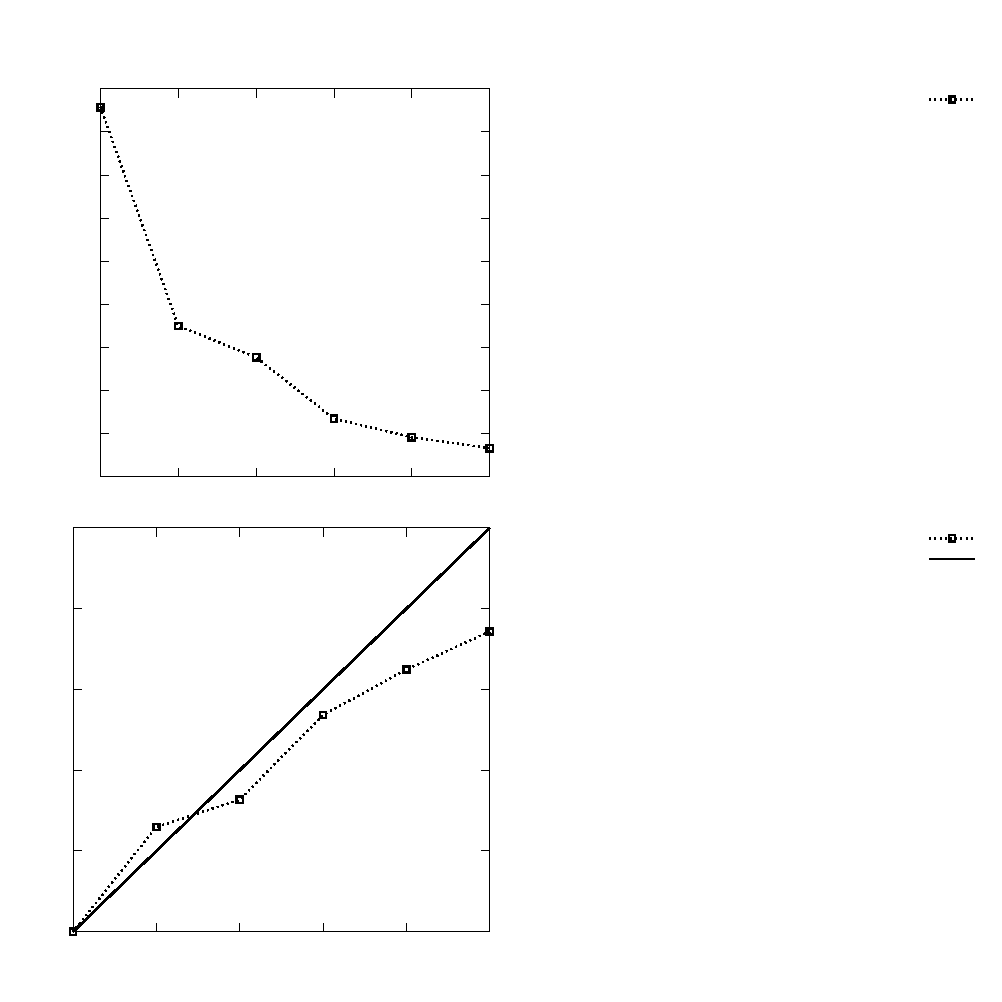
\includegraphics{MPIScalingTimes}}%
    \gplfronttext
  \end{picture}%
\endgroup

	\end{center}
	\caption{
		Solver runtime vs. processors, for polynomial degree $k=1/0$ leading to 212992 DoFs,
		for problem/Equation (\ref{eq:ContantCoeffPoissonBenchmark}).
	}
	\label{fig:Spherek1Time}
\end{figure}

\graphicspath{{./apdx-MPISolverPerformance/strongScaling/NSESphereComplex/plots/}}

\begin{figure}[h!]
	\begin{center}
		% GNUPLOT: LaTeX picture with Postscript
\begingroup
  \makeatletter
  \providecommand\color[2][]{%
    \GenericError{(gnuplot) \space\space\space\@spaces}{%
      Package color not loaded in conjunction with
      terminal option `colourtext'%
    }{See the gnuplot documentation for explanation.%
    }{Either use 'blacktext' in gnuplot or load the package
      color.sty in LaTeX.}%
    \renewcommand\color[2][]{}%
  }%
  \providecommand\includegraphics[2][]{%
    \GenericError{(gnuplot) \space\space\space\@spaces}{%
      Package graphicx or graphics not loaded%
    }{See the gnuplot documentation for explanation.%
    }{The gnuplot epslatex terminal needs graphicx.sty or graphics.sty.}%
    \renewcommand\includegraphics[2][]{}%
  }%
  \providecommand\rotatebox[2]{#2}%
  \@ifundefined{ifGPcolor}{%
    \newif\ifGPcolor
    \GPcolortrue
  }{}%
  \@ifundefined{ifGPblacktext}{%
    \newif\ifGPblacktext
    \GPblacktexttrue
  }{}%
  % define a \g@addto@macro without @ in the name:
  \let\gplgaddtomacro\g@addto@macro
  % define empty templates for all commands taking text:
  \gdef\gplbacktext{}%
  \gdef\gplfronttext{}%
  \makeatother
  \ifGPblacktext
    % no textcolor at all
    \def\colorrgb#1{}%
    \def\colorgray#1{}%
  \else
    % gray or color?
    \ifGPcolor
      \def\colorrgb#1{\color[rgb]{#1}}%
      \def\colorgray#1{\color[gray]{#1}}%
      \expandafter\def\csname LTw\endcsname{\color{white}}%
      \expandafter\def\csname LTb\endcsname{\color{black}}%
      \expandafter\def\csname LTa\endcsname{\color{black}}%
      \expandafter\def\csname LT0\endcsname{\color[rgb]{1,0,0}}%
      \expandafter\def\csname LT1\endcsname{\color[rgb]{0,1,0}}%
      \expandafter\def\csname LT2\endcsname{\color[rgb]{0,0,1}}%
      \expandafter\def\csname LT3\endcsname{\color[rgb]{1,0,1}}%
      \expandafter\def\csname LT4\endcsname{\color[rgb]{0,1,1}}%
      \expandafter\def\csname LT5\endcsname{\color[rgb]{1,1,0}}%
      \expandafter\def\csname LT6\endcsname{\color[rgb]{0,0,0}}%
      \expandafter\def\csname LT7\endcsname{\color[rgb]{1,0.3,0}}%
      \expandafter\def\csname LT8\endcsname{\color[rgb]{0.5,0.5,0.5}}%
    \else
      % gray
      \def\colorrgb#1{\color{black}}%
      \def\colorgray#1{\color[gray]{#1}}%
      \expandafter\def\csname LTw\endcsname{\color{white}}%
      \expandafter\def\csname LTb\endcsname{\color{black}}%
      \expandafter\def\csname LTa\endcsname{\color{black}}%
      \expandafter\def\csname LT0\endcsname{\color{black}}%
      \expandafter\def\csname LT1\endcsname{\color{black}}%
      \expandafter\def\csname LT2\endcsname{\color{black}}%
      \expandafter\def\csname LT3\endcsname{\color{black}}%
      \expandafter\def\csname LT4\endcsname{\color{black}}%
      \expandafter\def\csname LT5\endcsname{\color{black}}%
      \expandafter\def\csname LT6\endcsname{\color{black}}%
      \expandafter\def\csname LT7\endcsname{\color{black}}%
      \expandafter\def\csname LT8\endcsname{\color{black}}%
    \fi
  \fi
    \setlength{\unitlength}{0.0500bp}%
    \ifx\gptboxheight\undefined%
      \newlength{\gptboxheight}%
      \newlength{\gptboxwidth}%
      \newsavebox{\gptboxtext}%
    \fi%
    \setlength{\fboxrule}{0.5pt}%
    \setlength{\fboxsep}{1pt}%
\begin{picture}(9620.00,9620.00)%
    \gplgaddtomacro\gplbacktext{%
      \csname LTb\endcsname%
      \put(691,5057){\makebox(0,0)[r]{\strut{}$150$}}%
      \csname LTb\endcsname%
      \put(691,5429){\makebox(0,0)[r]{\strut{}$200$}}%
      \csname LTb\endcsname%
      \put(691,5801){\makebox(0,0)[r]{\strut{}$250$}}%
      \csname LTb\endcsname%
      \put(691,6172){\makebox(0,0)[r]{\strut{}$300$}}%
      \csname LTb\endcsname%
      \put(691,6544){\makebox(0,0)[r]{\strut{}$350$}}%
      \csname LTb\endcsname%
      \put(691,6916){\makebox(0,0)[r]{\strut{}$400$}}%
      \csname LTb\endcsname%
      \put(691,7288){\makebox(0,0)[r]{\strut{}$450$}}%
      \csname LTb\endcsname%
      \put(691,7660){\makebox(0,0)[r]{\strut{}$500$}}%
      \csname LTb\endcsname%
      \put(691,8031){\makebox(0,0)[r]{\strut{}$550$}}%
      \csname LTb\endcsname%
      \put(691,8403){\makebox(0,0)[r]{\strut{}$600$}}%
      \csname LTb\endcsname%
      \put(691,8775){\makebox(0,0)[r]{\strut{}$650$}}%
      \csname LTb\endcsname%
      \put(1335,4858){\makebox(0,0){\strut{}$10$}}%
      \csname LTb\endcsname%
      \put(1952,4858){\makebox(0,0){\strut{}$20$}}%
      \csname LTb\endcsname%
      \put(2569,4858){\makebox(0,0){\strut{}$30$}}%
      \csname LTb\endcsname%
      \put(3186,4858){\makebox(0,0){\strut{}$40$}}%
      \csname LTb\endcsname%
      \put(3804,4858){\makebox(0,0){\strut{}$50$}}%
      \csname LTb\endcsname%
      \put(4421,4858){\makebox(0,0){\strut{}$60$}}%
      \csname LTb\endcsname%
      \put(4756,5057){\makebox(0,0)[l]{\strut{} }}%
      \csname LTb\endcsname%
      \put(4756,5429){\makebox(0,0)[l]{\strut{} }}%
      \csname LTb\endcsname%
      \put(4756,5801){\makebox(0,0)[l]{\strut{} }}%
      \csname LTb\endcsname%
      \put(4756,6172){\makebox(0,0)[l]{\strut{} }}%
      \csname LTb\endcsname%
      \put(4756,6544){\makebox(0,0)[l]{\strut{} }}%
      \csname LTb\endcsname%
      \put(4756,6916){\makebox(0,0)[l]{\strut{} }}%
      \csname LTb\endcsname%
      \put(4756,7288){\makebox(0,0)[l]{\strut{} }}%
      \csname LTb\endcsname%
      \put(4756,7660){\makebox(0,0)[l]{\strut{} }}%
      \csname LTb\endcsname%
      \put(4756,8031){\makebox(0,0)[l]{\strut{} }}%
      \csname LTb\endcsname%
      \put(4756,8403){\makebox(0,0)[l]{\strut{} }}%
      \csname LTb\endcsname%
      \put(4756,8775){\makebox(0,0)[l]{\strut{} }}%
      \csname LTb\endcsname%
      \put(779,8974){\makebox(0,0){\strut{} }}%
      \csname LTb\endcsname%
      \put(1335,8974){\makebox(0,0){\strut{} }}%
      \csname LTb\endcsname%
      \put(1890,8974){\makebox(0,0){\strut{} }}%
      \csname LTb\endcsname%
      \put(2446,8974){\makebox(0,0){\strut{} }}%
      \csname LTb\endcsname%
      \put(3001,8974){\makebox(0,0){\strut{} }}%
      \csname LTb\endcsname%
      \put(3557,8974){\makebox(0,0){\strut{} }}%
      \csname LTb\endcsname%
      \put(4112,8974){\makebox(0,0){\strut{} }}%
      \csname LTb\endcsname%
      \put(4668,8974){\makebox(0,0){\strut{} }}%
    }%
    \gplgaddtomacro\gplfronttext{%
      \csname LTb\endcsname%
      \put(239,6916){\rotatebox{-270}{\makebox(0,0){\strut{}Time [s]}}}%
      \csname LTb\endcsname%
      \put(5030,6916){\rotatebox{-270}{\makebox(0,0){\strut{}SlvIter}}}%
      \csname LTb\endcsname%
      \put(2723,9472){\makebox(0,0){\strut{}Exclusive times}}%
      \csname LTb\endcsname%
      \put(8827,8675){\makebox(0,0)[r]{\strut{}Automatic MGLevels3}}%
      \csname LTb\endcsname%
      \put(8827,8476){\makebox(0,0)[r]{\strut{}SoftGMRES Swz w Coarse Overlap MGLevels3}}%
    }%
    \gplgaddtomacro\gplbacktext{%
      \csname LTb\endcsname%
      \put(691,684){\makebox(0,0)[r]{\strut{}$0.5$}}%
      \csname LTb\endcsname%
      \put(691,1169){\makebox(0,0)[r]{\strut{}$1$}}%
      \csname LTb\endcsname%
      \put(691,1654){\makebox(0,0)[r]{\strut{}$1.5$}}%
      \csname LTb\endcsname%
      \put(691,2138){\makebox(0,0)[r]{\strut{}$2$}}%
      \csname LTb\endcsname%
      \put(691,2623){\makebox(0,0)[r]{\strut{}$2.5$}}%
      \csname LTb\endcsname%
      \put(691,3108){\makebox(0,0)[r]{\strut{}$3$}}%
      \csname LTb\endcsname%
      \put(691,3593){\makebox(0,0)[r]{\strut{}$3.5$}}%
      \csname LTb\endcsname%
      \put(691,4077){\makebox(0,0)[r]{\strut{}$4$}}%
      \csname LTb\endcsname%
      \put(691,4562){\makebox(0,0)[r]{\strut{}$4.5$}}%
      \csname LTb\endcsname%
      \put(1335,485){\makebox(0,0){\strut{}$10$}}%
      \csname LTb\endcsname%
      \put(1952,485){\makebox(0,0){\strut{}$20$}}%
      \csname LTb\endcsname%
      \put(2569,485){\makebox(0,0){\strut{}$30$}}%
      \csname LTb\endcsname%
      \put(3186,485){\makebox(0,0){\strut{}$40$}}%
      \csname LTb\endcsname%
      \put(3804,485){\makebox(0,0){\strut{}$50$}}%
      \csname LTb\endcsname%
      \put(4421,485){\makebox(0,0){\strut{}$60$}}%
      \csname LTb\endcsname%
      \put(4756,684){\makebox(0,0)[l]{\strut{} }}%
      \csname LTb\endcsname%
      \put(4756,1169){\makebox(0,0)[l]{\strut{} }}%
      \csname LTb\endcsname%
      \put(4756,1654){\makebox(0,0)[l]{\strut{} }}%
      \csname LTb\endcsname%
      \put(4756,2138){\makebox(0,0)[l]{\strut{} }}%
      \csname LTb\endcsname%
      \put(4756,2623){\makebox(0,0)[l]{\strut{} }}%
      \csname LTb\endcsname%
      \put(4756,3108){\makebox(0,0)[l]{\strut{} }}%
      \csname LTb\endcsname%
      \put(4756,3593){\makebox(0,0)[l]{\strut{} }}%
      \csname LTb\endcsname%
      \put(4756,4077){\makebox(0,0)[l]{\strut{} }}%
      \csname LTb\endcsname%
      \put(4756,4562){\makebox(0,0)[l]{\strut{} }}%
      \csname LTb\endcsname%
      \put(779,4761){\makebox(0,0){\strut{} }}%
      \csname LTb\endcsname%
      \put(1335,4761){\makebox(0,0){\strut{} }}%
      \csname LTb\endcsname%
      \put(1890,4761){\makebox(0,0){\strut{} }}%
      \csname LTb\endcsname%
      \put(2446,4761){\makebox(0,0){\strut{} }}%
      \csname LTb\endcsname%
      \put(3001,4761){\makebox(0,0){\strut{} }}%
      \csname LTb\endcsname%
      \put(3557,4761){\makebox(0,0){\strut{} }}%
      \csname LTb\endcsname%
      \put(4112,4761){\makebox(0,0){\strut{} }}%
      \csname LTb\endcsname%
      \put(4668,4761){\makebox(0,0){\strut{} }}%
    }%
    \gplgaddtomacro\gplfronttext{%
      \csname LTb\endcsname%
      \put(239,2623){\rotatebox{-270}{\makebox(0,0){\strut{}Time [s]}}}%
      \csname LTb\endcsname%
      \put(5030,2623){\rotatebox{-270}{\makebox(0,0){\strut{}SlvInit}}}%
      \csname LTb\endcsname%
      \put(2723,187){\makebox(0,0){\strut{}Processors}}%
      \csname LTb\endcsname%
      \put(8827,4462){\makebox(0,0)[r]{\strut{}Automatic MGLevels3}}%
      \csname LTb\endcsname%
      \put(8827,4263){\makebox(0,0)[r]{\strut{}SoftGMRES Swz w Coarse Overlap MGLevels3}}%
    }%
    \gplbacktext
    \put(0,0){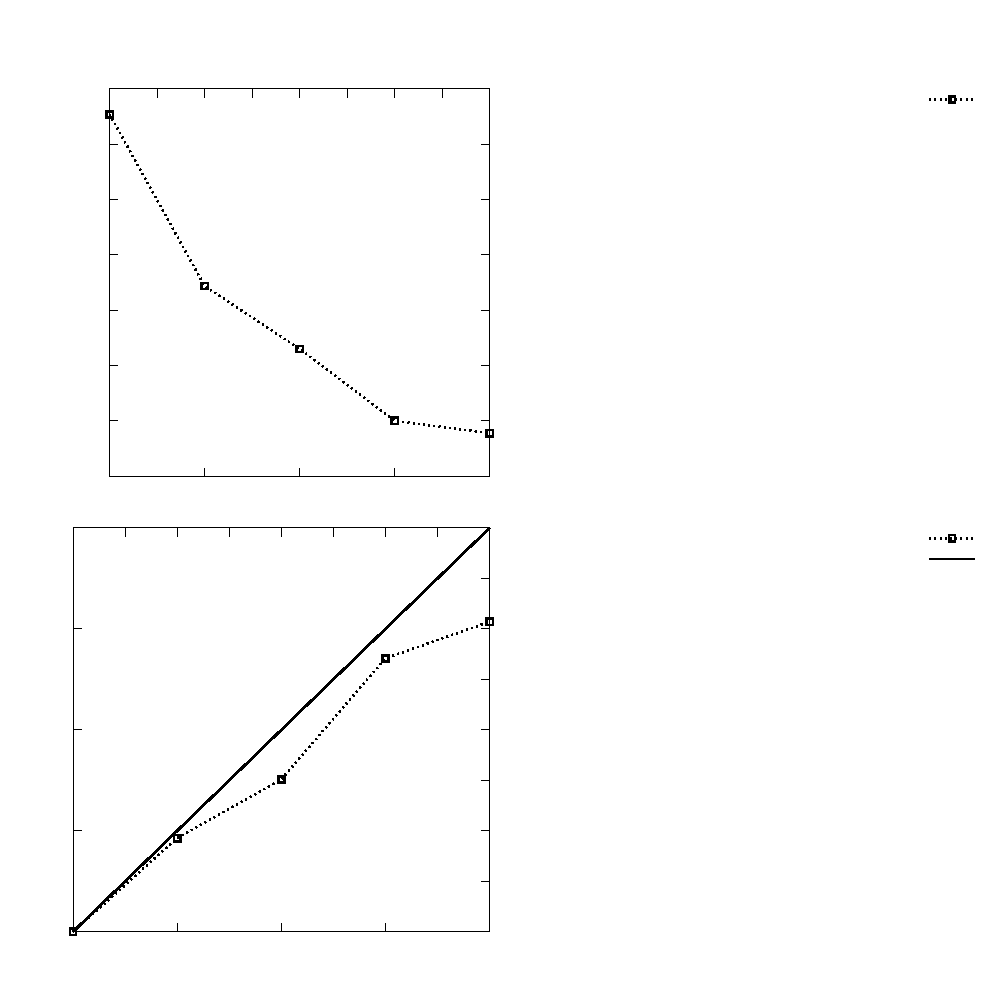
\includegraphics{MPIScalingTimes}}%
    \gplfronttext
  \end{picture}%
\endgroup

	\end{center}
	\caption{
		Solver runtime vs. processors, for polynomial degree $k=2/1$ leading to 557056 DoFs,
		for problem/Equation (\ref{eq:ContantCoeffPoissonBenchmark}).
	}
	\label{fig:Spherek1Time}
\end{figure}